% comparamos implemtaciones del mismo filtro (versión mas intuitiva posible de c vs asm con SIMD). Esto permite analizar mejor la optimizaciones del compilador. Sobre todo las de icc que tiene introducción automática de SIMD
% En todos los casos se realizó el gráfico C vs ASM (cantidad de clocks y cantidad de líneas de código).
% Como medimos. (menor vs promedio)
% Como se compiló. Compilamos con gcc, con icc, y con diferentes flags.
	% - (aclarar cuales y por qué)
	% - Explicar por qué se puso ICC y no otro(introduce SIMD automáticamente y se supone que es el compilador mas optimo para la arquitectura AMD-64 con procesadores intel).
% cómo se ejcutó. (Mínimas interrupciones, init 2 y kill -9 -1).
% Análisis del código. (object dump).
% - Los tres filtros se programaron pensando en minizar los accesos a memoria incluso en situaciones donde producía cálculo extra.

A la hora de implementar los filtros se tuvieron algunas consideraciones generales para mantener la coherencia dentro del trabajo y poder extraer resultados comparables entre los distintos filtros, como se detallan en los siguientes apartados.

\subsection{Criterios de implementación}

Para poder analizar de manera pura la diferencia entre los dos paradigmas, se procuró que las implementaciones en lenguaje C fueran lo mas intuitivas posibles; es decir, una traducción fiel a la descripción en lenguaje natural del comportamiento del filtro. No se utilizaron optimizaciones algorítmicas sofisticadas. Esto acarrea el beneficio adicional de simplificar la interpretación del código objeto generado por los compiladores, y les provee mayor libertad para realizar paralelización u otras optimizaciones sin necesariamente respetar el esquema planteado.

Por otro lado, todas las implementaciones en ASM se desarrollaron intentando minimizar los accesos a memoria, para evitar el cuello de botella de la arquitectura de Von Neumann. Una vez dentro del ciclo, sólo se accede a memoria para la lectura de la imagen fuente o la escritura de la imagen destino.

% (esto es medio un spoiler)
% Sin embargo en cada implementación se va a analizar si esto fue una decisión acertada o no.

\subsection{Compiladores utilizados}
			
Todos los programas en lenguaje C se compilaron con los siguientes compiladores:

\begin{itemize}
	\item GNU C Compiler (GCC): Se eligió por ser un compilador libre, conocido, popular, sumamente versatil y porque es capaz de realizar una gran gama de optimizacizaciones, probablemente todas aquellas que se pueden realizar sin acceder al micro código de Intel.

	\item Intel C++ Compiler (ICC): Este compilador realiza optimizaciones muy avanzadas aprovechando características detalladas de la microarquitectura Intel. Adicionalmente, introduce instrucciones de la familia de extensiones SSE de forma predeterminada; es decir, por defecto es capaz de generar código objeto manifestando paralelismo a nivel de datos.
\end{itemize} 
				
% esto no lo entiendo
Además si bien siempre se compiló indicándole al compilador que use instrucciones SSE4.2 además se hicieron 2 versiones distintas con cada compilador: Una con optimizaciones agresivas y otra sin ellas. Para la primera usó el flag -Ofast, mientras que para la segunda se dejó el comportamiento predeterminado.

\newpage

\subsection{Entorno de experimentación y método de medición}

A la hora de realizar las mediciones de tiempo, se intentó armar un entorno que introdujera la menor cantidad de ruido adicional como fuera posible. Por esta razón, antes de realizar las experiencias se terminaron todas las aplicaciones no vitales para el sistema operativo, incluída la interfaz gráfica y acceso a internet. \footnote{Comandos \emph{init 1} y \emph{kill -9 -1} en Linux.}. Además, se desconectaron los periféricos
innecesarios.

De todas formas, la interacción con el sistema operativo es insoslayable, y algunas mediciones mostraron valores mucho mayores a la media, presumiblemente debido a interrupciones. Como criterio de eliminación de valores atípicos, se utilizó el procedimiento estándar de descartar mediciones con valores por debajo de $Q_1 - 1.5 * IQR$ o por encima de $Q_3 + 1.5 * IQR$, donde $Q_1$ y $Q_3$ son el primer y tercer cuartil de los datos, respectivamente, e $IQR$ es el rango intercuartil o $Q_3 - Q_1$ (ver figura \ref{fig:cuariles}).

Las mediciones se repitieron entre 50 y 100 veces según el filtro, eligiendo esta cantidad en base a prueba y error de forma tal que la variación de la media fuera despreciable. Finalmente, se tomó el valor de la media como representante de los conjuntos de mediciones para realizar comparaciones entre distintas implementaciones, siendo esta una buena medida dada la baja variación en los datos obtenidos luego de filtrar los valores atípicos (en general, menos del 2\%).
% le voy a enchufar otra fotito aca
\begin{figure}[h!]
\begin{center}
  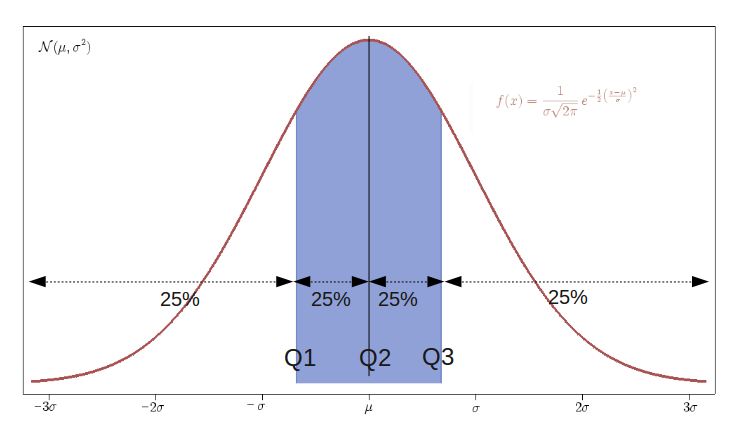
\includegraphics[scale=0.5]{secciones/consideraciones/imagenes/cuartiles.png}
\end{center}
\caption{Gráfico representando el rango intercuartil (sombreado), y el rango de valores aceptados.}
\label{fig:cuariles}
\end{figure}
	

	

